\documentclass[12pt]{article}

\usepackage{sbc-template}
\usepackage{graphicx,url}
\usepackage[utf8]{inputenc}
\usepackage[brazil]{babel}
\usepackage{amsmath}
\usepackage{booktabs}
\usepackage{xcolor}
\usepackage{float}

\sloppy

% Marcador para o que ainda precisa ser preenchido (aparece em vermelho no PDF)
\newcommand{\todo}[1]{\textcolor{red}{\textbf{[#1]}}}

\title{Programação Paralela com \textit{Threads}: Produto Escalar, Multiplicação de Matrizes e um Jogo no Estilo \textit{Asteroids}}

\author{Beatriz Quaresma Athaide\inst{1}, Ruthelene Rodrigues Farias\inst{1},
Jonathas Monteiro da Trindade\inst{1}\\
% \todo{Leticia: incluir sobrenome completo e e-mail se ela constar como autora}
}

\address{Instituto de Computação -- Universidade Federal do Amazonas (UFAM)\\
Manaus -- AM -- Brasil
\email{\{beatriz.quaresma,ruthelene.farias,jonathas.trindade\}@icomp.ufam.edu.br}
}

\begin{document}

\maketitle

\begin{abstract}
This report presents the results of Practical Assignment 2 of the Operating Systems course, which explores parallel programming with threads in C using the POSIX \textit{pthread} library. We implemented sequential and parallel versions of the dot product and of matrix multiplication, evaluating execution time and speedup on different CPUs and thread counts. We also developed a multithreaded game inspired by \textit{Asteroids} to illustrate the use of threads in interactive applications. \todo{Revisar o abstract ao final com os principais resultados.}
\end{abstract}

\begin{resumo}
Este relatório apresenta os resultados do Trabalho Prático 2 da disciplina de Sistemas Operacionais, que explora a programação paralela com \textit{threads} em C por meio da biblioteca \textit{pthread}. Foram implementadas versões sequencial e paralela do produto escalar e da multiplicação de matrizes, avaliando-se o tempo de execução e a aceleração (\textit{speedup}) em diferentes CPUs e quantidades de \textit{threads}. Também foi desenvolvido um jogo multithread inspirado em \textit{Asteroids} para ilustrar o uso de \textit{threads} em aplicações interativas. \todo{Revisar o resumo ao final com os principais resultados.}
\end{resumo}

%==========================================================
\section{Introdução}
\label{sec:intro}

O objetivo deste trabalho é proporcionar experiência prática com o uso de \textit{threads} para processamento paralelo. O trabalho é composto por três questões: (1) produto escalar entre dois vetores; (2) multiplicação de duas matrizes; e (3) uma aplicação simulada, na qual o uso de \textit{threads} traz vantagens, escolhida pela equipe como um jogo no estilo \textit{Asteroids}.

Todas as implementações foram feitas em linguagem C com a biblioteca \textit{pthread}~\cite{butenhof1997}. Para as questões 1 e 2, a métrica de desempenho utilizada é a aceleração (\textit{speedup}), definida como
\begin{equation}
S_p = \frac{T_s}{T_p},
\end{equation}
em que $T_s$ é o tempo de execução da versão sequencial e $T_p$ é o tempo da versão paralela com $p$ \textit{threads}. Também é reportada a eficiência $E_p = S_p / p$.

As seções seguintes descrevem o ambiente e a metodologia de medição (Seção~\ref{sec:metodo}), cada uma das questões (Seções~\ref{sec:q1}, \ref{sec:q2} e~\ref{sec:q3}) e as conclusões (Seção~\ref{sec:conclusao}). As fontes consultadas, incluindo o uso de inteligência artificial, estão registradas na Seção~\ref{sec:fontes}.

%==========================================================
\section{Ambiente Experimental e Metodologia de Medição}
\label{sec:metodo}

Para que os resultados das diferentes máquinas fossem comparáveis, a equipe adotou o mesmo padrão de medição em todos os experimentos:

\begin{itemize}
  \item Linguagem C compilada com \texttt{gcc -O2 -pthread};
  \item Tempo medido com \texttt{clock\_gettime(CLOCK\_MONOTONIC)}, considerando apenas a região de cálculo (sem a alocação e inicialização dos dados);
  \item Cada configuração foi executada \textbf{5 vezes} e é reportada a média dos tempos;
  \item Os dados de entrada são gerados de forma determinística, de modo que todas as versões operam sobre os mesmos valores;
  \item A correção das versões paralelas foi verificada comparando um \textit{checksum} do resultado com o da versão sequencial.
\end{itemize}

A Tabela~\ref{tab:maquinas} apresenta as máquinas utilizadas nos experimentos das Questões 1 e 2.

\begin{table}[H]
\centering
\caption{Computadores utilizados nos experimentos.}
\label{tab:maquinas}
\begin{tabular}{llccl}
\toprule
\textbf{Máquina} & \textbf{Processador} & \textbf{Núcleos} & \textbf{Núcleos lógicos} & \textbf{SO} \\
\midrule
Beatriz     & \todo{modelo da CPU} & \todo{n} & \todo{n} & \todo{SO} \\
Ruthelene   & \todo{modelo da CPU} & \todo{n} & \todo{n} & \todo{SO} \\
Jonathas    & \todo{modelo da CPU} & \todo{n} & \todo{n} & \todo{SO} \\
Leticia     & \todo{modelo da CPU} & \todo{n} & \todo{n} & \todo{SO} \\
\bottomrule
\end{tabular}
\end{table}

%==========================================================
\section{Questão 1: Produto Escalar}
\label{sec:q1}
% Responsável: Ruthelene

\subsection{Descrição da solução}
\todo{Ruthelene: descrever o algoritmo sequencial e o paralelo. Explicar como o vetor é dividido entre as \textit{threads}, como as somas parciais são combinadas (por exemplo, cada \textit{thread} calcula uma soma parcial em uma posição própria de um vetor e a \textit{thread} principal soma tudo após o \texttt{pthread\_join}, evitando \textit{mutex} e condições de corrida) e como o usuário informa o número de \textit{threads}.}

\subsection{Resultados}
\todo{Tamanhos de vetor testados (de milhares a milhões de elementos) e quantidades de \textit{threads}.}

\begin{figure}[H]
\centering
% \includegraphics[width=.8\textwidth]{figuras/q1_tempo_vs_tamanho.png}
\fbox{\parbox{.8\textwidth}{\centering \todo{Gráfico com duas curvas: tempo de execução $\times$ tamanho do vetor, para o programa sequencial e o paralelo}}}
\caption{Tempo de execução em função do tamanho do vetor (sequencial vs. paralelo).}
\label{fig:q1-tempo}
\end{figure}

\begin{table}[H]
\centering
\caption{Questão 1: tempo médio (s) e \textit{speedup} por máquina e número de \textit{threads}.}
\label{tab:q1}
\begin{tabular}{llrrrr}
\toprule
\textbf{Máquina} & \textbf{Threads} & \textbf{Tamanho} & \textbf{$T_s$ (s)} & \textbf{$T_p$ (s)} & \textbf{$S_p$} \\
\midrule
\todo{...} & \todo{...} & \todo{...} & \todo{...} & \todo{...} & \todo{...} \\
\bottomrule
\end{tabular}
\end{table}

\subsection{Análise}
\todo{Impacto das diferentes CPUs no tempo de execução, comportamento do \textit{speedup} ao variar as \textit{threads}, e o que acontece quando há mais \textit{threads} que núcleos.}

%==========================================================
\section{Questão 2: Multiplicação de Matrizes}
\label{sec:q2}
% Responsável: Beatriz

\subsection{Descrição da solução}

Foram desenvolvidos dois programas para o cálculo de $C = A \times B$, com matrizes quadradas $N \times N$ de números de ponto flutuante de dupla precisão (\texttt{double}): \texttt{matmul\_seq.c}, a versão sequencial, e \texttt{matmul\_par.c}, a versão paralela com \textit{pthreads}, na qual o número de \textit{threads} é informado pelo usuário na linha de comando. As matrizes são armazenadas em vetores unidimensionais, linha a linha.

\paragraph{Versão sequencial.} Foram implementadas duas ordens dos laços: a clássica \texttt{ijk}, em que cada elemento $C_{ij}$ é obtido pelo produto escalar da linha $i$ de $A$ com a coluna $j$ de $B$; e a ordem \texttt{ikj}, em que, para cada elemento $A_{ik}$, a linha $k$ de $B$ é percorrida sequencialmente, acumulando em $C_{i\cdot}$. Na ordem \texttt{ijk} a matriz $B$ é acessada por colunas, o que degrada o aproveitamento da memória \textit{cache}; na ordem \texttt{ikj} todos os acessos são sequenciais. Ambas produzem exatamente o mesmo resultado, pois a ordem de acumulação sobre $k$ é a mesma para cada elemento de $C$.

\paragraph{Versão paralela.} Como cada elemento de $C$ pode ser calculado de forma independente, não há dependência de dados entre as \textit{threads}: cada uma escreve apenas em posições distintas de $C$ e somente lê $A$ e $B$. Assim, não é necessário o uso de \textit{mutex} ou outros mecanismos de sincronização, apenas a criação (\texttt{pthread\_create}) e a espera (\texttt{pthread\_join}) das \textit{threads}. Com $T$ \textit{threads}, foram implementadas três estratégias de divisão de tarefas:

\begin{enumerate}
  \item \textbf{Linhas contíguas}: as $N$ linhas de $C$ são divididas em $T$ faixas consecutivas de tamanho aproximadamente igual;
  \item \textbf{Linhas cíclicas}: a \textit{thread} $t$ calcula as linhas $t, t+T, t+2T, \ldots$, o que melhora o balanceamento de carga quando $N$ não é múltiplo de $T$;
  \item \textbf{Blocos}: a matriz $C$ é dividida em blocos (\textit{tiles}) de $BS \times BS$ elementos, distribuídos ciclicamente entre as \textit{threads}, com $BS$ configurável.
\end{enumerate}

Cada estratégia pode ser combinada com as duas ordens de laços (\texttt{ijk} e \texttt{ikj}), resultando em seis variantes paralelas. O código-fonte e os \textit{scripts} de experimentos estão no pacote entregue (pasta \texttt{q2/}).

\subsection{Metodologia dos experimentos}

Foram executados, em cada máquina da Tabela~\ref{tab:maquinas}, todos os experimentos do \textit{script} \texttt{run\_bench.sh}, que varia:
\begin{itemize}
  \item o tamanho das matrizes: $N \in \{200, 400, 600, 800, 1000, 1500, 2000\}$ \todo{ajustar se a lista mudou};
  \item o número de \textit{threads}: 1, 2, 4, o número de núcleos lógicos da máquina e o dobro desse valor;
  \item a estratégia de divisão (linhas, cíclica, blocos) e a ordem dos laços (\texttt{ijk}, \texttt{ikj});
  \item o tamanho do bloco $BS \in \{16, 32, 64, 128, 256\}$ para a estratégia de blocos.
\end{itemize}
O tempo $T_s$ usado no cálculo do \textit{speedup} é o da \textbf{melhor} versão sequencial (menor tempo entre \texttt{ijk} e \texttt{ikj}) para o mesmo $N$, de modo a não inflar a aceleração comparando com uma versão sequencial ineficiente. Também foi calculado o \textit{speedup} em relação à versão sequencial com a mesma ordem de laços, para isolar o ganho devido exclusivamente ao paralelismo.

\subsection{Resultados}

\begin{figure}[H]
\centering
% 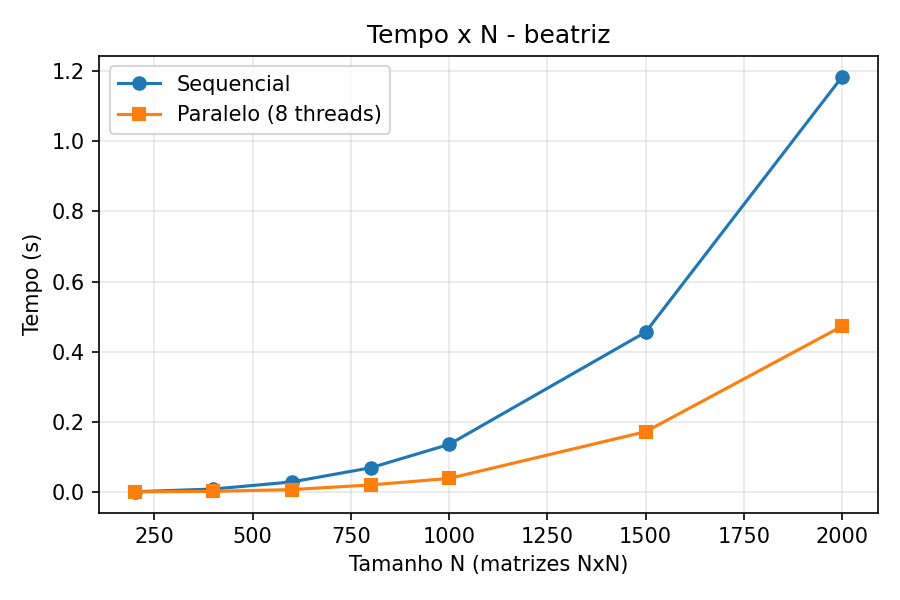
\includegraphics[width=.8\textwidth]{figuras/grafico_tempo_beatriz.png}
\fbox{\parbox{.8\textwidth}{\centering \todo{inserir grafico\_tempo\_<maquina>.png gerado por analyze.py}}}
\caption{Questão 2: tempo de execução $\times$ tamanho da matriz.}
\label{fig:q2-tempo}
\end{figure}

\begin{figure}[H]
\centering
% 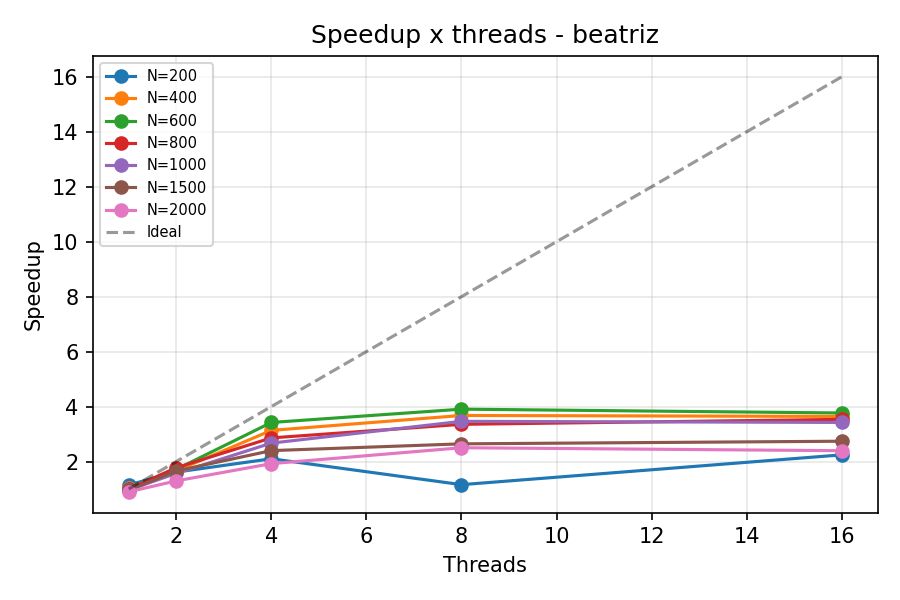
\includegraphics[width=.8\textwidth]{figuras/grafico_speedup_beatriz.png}
\fbox{\parbox{.8\textwidth}{\centering \todo{inserir grafico\_speedup\_<maquina>.png gerado por analyze.py}}}
\caption{Questão 2: \textit{speedup} em função do número de \textit{threads}.}
\label{fig:q2-speedup}
\end{figure}

\begin{table}[H]
\centering
\caption{Questão 2: \textit{speedup} da melhor configuração paralela para $N=\todo{N}$, por máquina e número de \textit{threads} ($n_c$ = número de núcleos lógicos).}
\label{tab:q2-speedup}
\begin{tabular}{lrrrrr}
\toprule
\textbf{Máquina} & \textbf{1} & \textbf{2} & \textbf{4} & \textbf{$n_c$} & \textbf{$2n_c$} \\
\midrule
Beatriz   & \todo{} & \todo{} & \todo{} & \todo{} & \todo{} \\
Ruthelene & \todo{} & \todo{} & \todo{} & \todo{} & \todo{} \\
Jonathas  & \todo{} & \todo{} & \todo{} & \todo{} & \todo{} \\
Leticia   & \todo{} & \todo{} & \todo{} & \todo{} & \todo{} \\
\bottomrule
\end{tabular}
\end{table}

\begin{table}[H]
\centering
\caption{Questão 2: comparação das estratégias de divisão ($N=\todo{N}$, $T=\todo{T}$ \textit{threads}, máquina \todo{máquina}).}
\label{tab:q2-estrategias}
\begin{tabular}{llrrr}
\toprule
\textbf{Estratégia} & \textbf{Ordem} & \textbf{Tempo (s)} & \textbf{$S_p$} & \textbf{$E_p$} \\
\midrule
Linhas contíguas & \texttt{ijk} & \todo{} & \todo{} & \todo{} \\
Linhas contíguas & \texttt{ikj} & \todo{} & \todo{} & \todo{} \\
Linhas cíclicas  & \texttt{ijk} & \todo{} & \todo{} & \todo{} \\
Linhas cíclicas  & \texttt{ikj} & \todo{} & \todo{} & \todo{} \\
Blocos ($BS=\todo{}$) & \texttt{ijk} & \todo{} & \todo{} & \todo{} \\
Blocos ($BS=\todo{}$) & \texttt{ikj} & \todo{} & \todo{} & \todo{} \\
\bottomrule
\end{tabular}
\end{table}

\subsection{Análise}

\todo{Beatriz: após rodar os experimentos, discutir os pontos abaixo com os números reais.}
\begin{itemize}
  \item \textbf{Melhor configuração encontrada:} qual combinação de estratégia, ordem dos laços, tamanho de bloco e número de \textit{threads} obteve o menor tempo, e com qual \textit{speedup}.
  \item \textbf{Efeito da ordem dos laços:} diferença de tempo entre \texttt{ijk} e \texttt{ikj} na versão sequencial e sua relação com o uso da \textit{cache}.
  \item \textbf{Efeito da estratégia de divisão:} se a divisão por linhas contíguas, cíclica ou por blocos foi mais vantajosa e por quê (balanceamento de carga, localidade de \textit{cache}).
  \item \textbf{Número de \textit{threads} versus núcleos:} comportamento do \textit{speedup} ao passar do número de núcleos (custo de criação e troca de contexto das \textit{threads}, \textit{hyper-threading}).
  \item \textbf{Impacto das diferentes CPUs:} comparação entre as máquinas, relacionando com número de núcleos, frequência e tamanho de \textit{cache}.
  \item \textbf{Eficiência:} por que o \textit{speedup} fica abaixo do ideal (limitação de largura de banda de memória, \textit{overhead} de criação das \textit{threads}, parte sequencial do programa).
  \item \textbf{Efeito do tamanho do problema:} para matrizes pequenas o \textit{overhead} pode superar o ganho; a partir de qual $N$ o paralelismo compensa.
\end{itemize}

%==========================================================
\section{Questão 3: Jogo no Estilo \textit{Asteroids}}
\label{sec:q3}
% Responsáveis: Leticia e Jonathas

\subsection{Aplicação escolhida}
\todo{Leticia e Jonathas: apresentar o jogo, o objetivo e a aprovação do professor (data e forma de comunicação). Registrar que a aplicação foi alterada em relação às ideias iniciais da equipe (editor de texto e navegador \textit{web}).}

\subsection{Ideia e arquitetura do sistema}
\todo{Descrever as entidades do jogo (nave, asteroides, tiros) e como são mapeadas em \textit{threads}. Sugestão: \textit{thread} de entrada do teclado, \textit{threads} dos asteroides, \textit{threads} dos tiros, \textit{thread} de detecção de colisões e \textit{thread} de renderização.}

\begin{figure}[H]
\centering
\fbox{\parbox{.8\textwidth}{\centering \todo{Diagrama da arquitetura: \textit{threads}, dados compartilhados e \textit{mutexes}}}}
\caption{Arquitetura do jogo e relação entre as \textit{threads}.}
\label{fig:q3-arq}
\end{figure}

\subsection{Sincronização}
\todo{Descrever quais estruturas compartilhadas existem (lista de entidades, placar, vidas), quais \textit{mutexes}/variáveis de condição protegem cada uma e quais condições de corrida foram evitadas.}

\subsection{Decisões para demonstrar o uso das \textit{threads}}
\todo{Parâmetros de entrada (número de \textit{threads}, de asteroides, dificuldade), comandos interativos, uso de \texttt{sleep} para diferenciar velocidades e os \textit{prints} que identificam cada \textit{thread} (exemplo de saída).}

\subsection{Versão sequencial equivalente e avaliação de desempenho}
\todo{Descrever a versão sem \textit{threads} (laço único de jogo). Se houver comparação de desempenho (por exemplo, simulação sem renderização com muitos asteroides), apresentar tempos e \textit{speedup} em tabela. Se o foco não for desempenho, discutir as funcionalidades que a versão sequencial não permite, como responder ao teclado enquanto os objetos se movem de forma independente.}

%==========================================================
\section{Conclusão}
\label{sec:conclusao}

\todo{Escrever ao final, com base nos resultados reais. Pontos sugeridos: (i) ganhos de \textit{speedup} obtidos nas Questões 1 e 2 e suas limitações; (ii) influência da arquitetura da CPU; (iii) o que a Questão 3 mostrou sobre sincronização e concorrência; (iv) dificuldades e aprendizados da equipe.}

%==========================================================
\section{Registro de Fontes}
\label{sec:fontes}

Conforme exigido no enunciado, registramos as fontes utilizadas no desenvolvimento do trabalho:

\begin{itemize}
  \item \textbf{Inteligência artificial:} o assistente Claude (Anthropic)~\cite{claude} foi utilizado para auxiliar na estruturação e escrita do código da Questão 2 (\texttt{matmul\_seq.c}, \texttt{matmul\_par.c}, \texttt{common.h}), dos \textit{scripts} de experimentos (\texttt{run\_bench.sh}, \texttt{analyze.py}) e na elaboração do esqueleto deste relatório. O código foi compilado, testado e revisado pela equipe. \todo{Cada integrante deve acrescentar aqui o uso de IA, sites ou livros em suas próprias partes (Q1 e Q3).}
  \item \textbf{Livros e materiais de referência:} \cite{tanenbaum2014,silberschatz2018,pacheco2011,butenhof1997}.
  \item \textbf{Slides e material da disciplina:} \todo{listar, se utilizados}.
  \item \textbf{URLs:} \todo{listar, se utilizadas}.
\end{itemize}

\bibliographystyle{sbc}
\bibliography{refs}

\end{document}
